%%%%%%%%%%%%%%%%%%%%%%%%%%%%%%%%%%%%%%%%%%%%%%%%%%%%%%%%%%%%%%%%%%%%%%%%%%%%%%%
\section{Results}
\label{sec:results}
%%%%%%%%%%%%%%%%%%%%%%%%%%%%%%%%%%%%%%%%%%%%%%%%%%%%%%%%%%%%%%%%%%%%%%%%%%%%%%%

Both benchmarks were modeled with OpenMOC using MGXS generated by OpenMC for the null and degenerate spatial homogenization schemes. The eigenvalues and pin-wise fission and U-238 capture rates computed by OpenMOC are compared to the reference OpenMC solutions in \autoref{subsec:eigenvalues}, \autoref{subsec:fiss-rates} and \autoref{subsec:capt-rates}, respectively.


%%%%%%%%%%%%%%%%%%%%%%%%%%%%%%%%%%%%%%%%%%%%%%%%%%%%%%%%%%%%%%%%%%%%%%%%%%%%%%%
\subsection{Eigenvalues}
\label{subsec:eigenvalues}

The OpenMOC eigenvalues were compared to the reference OpenMC eigenvalues from \autoref{tab:keff-reference}. The eigenvalue bias $\Delta\rho$ was calculated by comparing the eigenvalue $k_{eff}^{MOC}$ from OpenMOC to the reference eigenvalue $k_{eff}^{MC}$ computed by OpenMC in units of per cent mille (pcm):

\begin{equation}
\label{eqn:delta-rho}
\Delta\rho = \left(k_{eff}^{MOC} - k_{eff}^{MC}\right) \times 10^{5}
\end{equation}

The bias is listed for both benchmarks and spatial homogenization schemes in \autoref{tab:keff-bias}. The slightly negative bias of a few hundred pcm is likely due to the flux separability approximation \citep{boyd2018sph}, which permits use of the scalar rather than the angular neutron flux to collapse cross sections. The eigenvalues for the null and degenerate schemes are identical for the fuel assembly and are consistent to within 10 pcm for the colorset benchmark. As these results show, the choice of null or degenerate spatial homogenization schemes is inconsequential to the eigenvalue predictions. This is to be expected since the two methods uses the same MC flux to collapse the MGXS and preserve global reactivity.

%It should be recalled that isotropic in lab scattering is used by OpenMC to compute both the reference solution and the MGXS. If anisotropic scattering were employed in OpenMC, one would expect quite different biases without a robust implementation of a higher order scattering kernel in OpenMOC.

\begin{table}[h!]
  \centering
  \caption{OpenMOC eigenvalue bias $\Delta\rho$.}
  \label{tab:keff-bias} 
  \begin{tabular}{l c c}
  \toprule
  \textbf{Benchmark} & \textbf{Null} & \textbf{Degenerate} \\
  \midrule
  Assembly & -161 & -161 \\
  Colorset & -142 & -132 \\
  \bottomrule
\end{tabular}
\end{table}


%%%%%%%%%%%%%%%%%%%%%%%%%%%%%%%%%%%%%%%%%%%%%%%%%%%%%%%%%%%%%%%%%%%%%%%%%%%%%%%
\subsection{Fission Rates}
\label{subsec:fiss-rates}

The OpenMOC energy-integrated pin-wise fission rates were compared to the reference OpenMC fission rates shown in \autoref{fig:fiss-assm} and \autoref{fig:fiss-reflector}. The percent relative errors for each pin's fission rates were computed and the maximum and mean errors are listed for both benchmarks and spatial homogenization schemes in \autoref{tab:fiss-errors}. In particular, the maximum errors are the maximum of the absolute values of the errors along with the appropriate sign, while the mean errors are the averages of the absolute error magnitudes. The fission rate errors are somewhat dependent on the spatial homogenization scheme used to compute MGXS in the fuel. In particular, the degenerate scheme produces slightly smaller maximum and mean errors than the null scheme.

\begin{table}[h!]
  \centering
  \caption{OpenMOC fission rate percent relative errors.}
  \label{tab:fiss-errors}
  \begin{tabular}{l l r r}
  \toprule
  \textbf{Benchmark} & \textbf{Metric} & \textbf{Null} & \textbf{Degenerate} \\
  \midrule
  \multirow{2}{*}{Assembly} & Max  & 0.380 & 0.315 \\
                            & Mean & 0.074 & 0.079 \\
  \midrule
  \multirow{2}{*}{Colorset} & Max  & 0.764 & 0.602 \\
                            & Mean & 0.178 & 0.138 \\
  \bottomrule
\end{tabular}
\end{table}

The spatial distributions of fission rate errors are plotted as heatmaps for each benchmark in \autoref{fig:fiss-errors}. The heatmaps illustrate systematic trends in the pin-wise fission errors which correlate with spatial heterogeneities in each benchmark. In particular, the fission rates are generally underpredicted for pins adjacent to a single CRGT, but overpredicted for pins adjacent to two CRGTs in the assembly. In addition, the errors are largest for pins along the inter-assembly and assembly-reflector interfaces for the colorset benchmark.

%For the PWR benchmarks modeled here, the moderation provided by neighboring CRGTs and reflectors softens the flux for nearby fuel pins and should be modeled when collapsing pin-wise MGXS for high-fidelity multi-group transport calculations.

\begin{figure*}[h!]
\centering
\begin{subfigure}{0.45\textwidth}
  \centering
  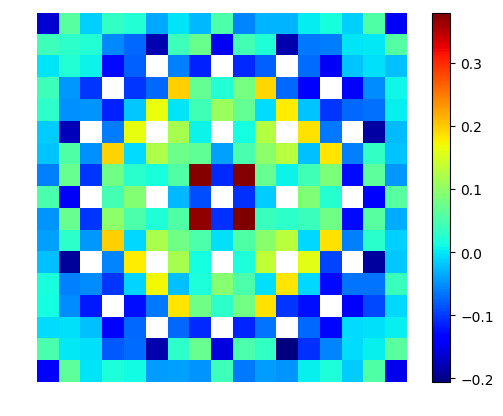
\includegraphics[width=\linewidth]{figures/assembly/fiss-null-errors}
  \caption{}
  \label{fig:assm-fiss-null-error}
\end{subfigure}%
\begin{subfigure}{0.45\textwidth}
  \centering
  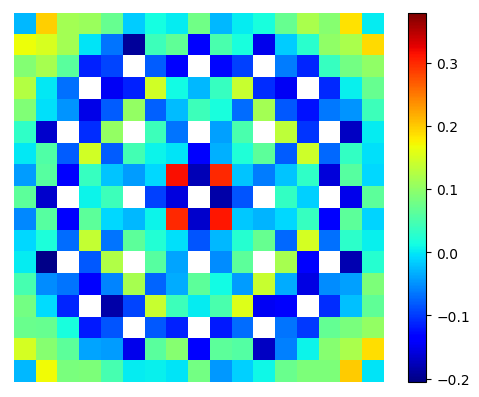
\includegraphics[width=\linewidth]{figures/assembly/fiss-degenerate-errors}
  \caption{}
  \label{fig:assm-fiss-degen-error}
\end{subfigure}
\begin{subfigure}{0.45\textwidth}
  \centering
  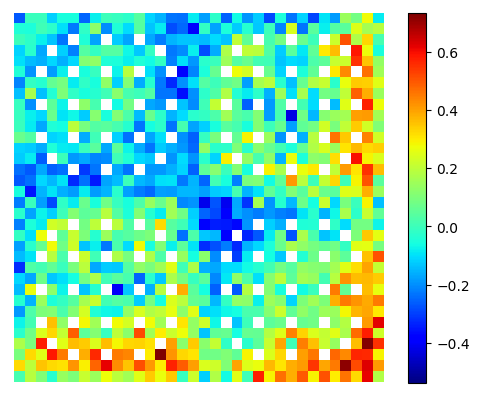
\includegraphics[width=\linewidth]{figures/reflector/fiss-null-errors}
  \caption{}
  \label{fig:reflector-fiss-null-error}
\end{subfigure}%
\begin{subfigure}{0.45\textwidth}
  \centering
  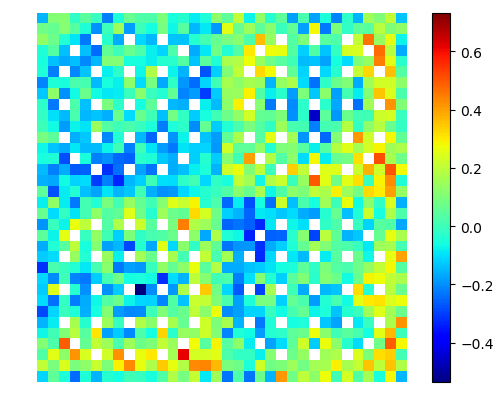
\includegraphics[width=\linewidth]{figures/reflector/fiss-degenerate-errors}
  \caption{}
  \label{fig:reflector-fiss-degen-error}
\end{subfigure}
\caption{OpenMOC fission rate percent relative errors for the assembly (a) and colorset (b) benchmarks.}
\label{fig:fiss-errors}
\end{figure*}


%%%%%%%%%%%%%%%%%%%%%%%%%%%%%%%%%%%%%%%%%%%%%%%%%%%%%%%%%%%%%%%%%%%%%%%%%%%%%%%
\subsection{Capture Rates}
\label{subsec:capt-rates}

The OpenMOC energy-integrated pin-wise U-238 capture rates were compared to the reference OpenMC capture rates shown in \autoref{fig:capt-assm} and \autoref{fig:capt-reflector}. The percent relative errors for each pin's capture rates were computed and the maximum and mean errors are listed for both benchmarks and spatial homogenization schemes in \autoref{tab:capt-errors}. In particular, the maximum errors are the maximum of the absolute values of the errors along with the appropriate sign, while the mean errors are the averages of the absolute error magnitudes. The capture rate errors are more dependent on the spatial homogenization scheme used to compute MGXS in the fuel than are the fission rate errors. In particular, the degenerate scheme produces much smaller maximum and mean errors than the null scheme. The maximum error is greater than 1\% for both benchmarks with the null scheme, but is reduced by 2 -- 5$\times$ with the use of degenerate homogenization.

\begin{table}[h!]
  \centering
  \caption{OpenMOC U-238 capture rate percent relative errors.}
  \label{tab:capt-errors} 
  \begin{tabular}{l l r r}
  \toprule
  \textbf{Benchmark} & \textbf{Metric} & \textbf{Null} & \textbf{Degenerate} \\
  \midrule
  \multirow{2}{*}{Assembly} & Max  & -1.101 &  0.386 \\
                            & Mean &  0.479 &  0.086 \\
  \midrule
  \multirow{2}{*}{Colorset} & Max  & -1.969 & -0.783 \\
                            & Mean &  0.478 &  0.165 \\
  \bottomrule
\end{tabular}
\end{table}

The spatial distributions of capture rate errors are plotted as heatmaps for each benchmark in \autoref{fig:capt-errors}. The heatmaps illustrate systematic error trends in the pin-wise capture errors which correlate with spatial heterogeneities in each benchmark. The capture rate errors are most significant for pins adjacent to CRGTs and along the inter-assembly and assembly-reflector interfaces. In addition, the heatmaps illustrate how degenerate spatial homogenization scheme ``smooths'' the pin-wise errors as compared to the null scheme. In particular, the differential of the errors for pins near CRGTs and BPs, and along inter-assembly and assembly-reflector interfaces is substantially reduced when degenerate homogenization is applied. This underscores the importance of accounting for spatial heterogeneities -- such as the added moderation from CRGTs and reflectors -- when generating MGXS to predict U-238 capture and Pu-239 production in LWRs. The moderation provided by neighboring CRGTs and/or reflectors softens the local flux for nearby fuel pins and should be modeled when collapsing pin-wise MGXS for high-fidelity multi-group transport calculations. 

\begin{figure*}[h!]
\centering
\begin{subfigure}{0.45\textwidth}
  \centering
  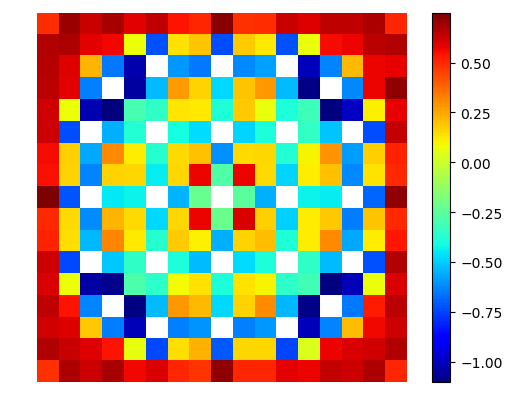
\includegraphics[width=\linewidth]{figures/assembly/capt-null-errors}
  \caption{}
  \label{fig:assm-capt-null-error}
\end{subfigure}%
\begin{subfigure}{0.45\textwidth}
  \centering
  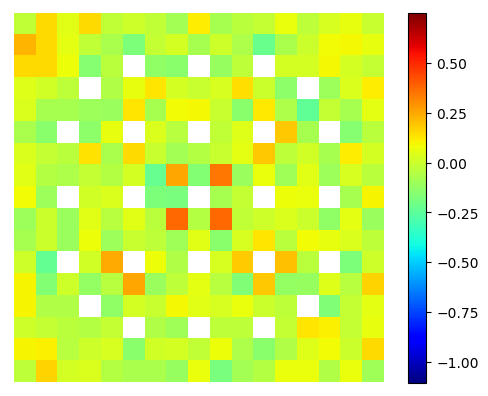
\includegraphics[width=\linewidth]{figures/assembly/capt-degenerate-errors}
  \caption{}
  \label{fig:assm-capt-degen-error}
\end{subfigure}
\begin{subfigure}{0.45\textwidth}
  \centering
  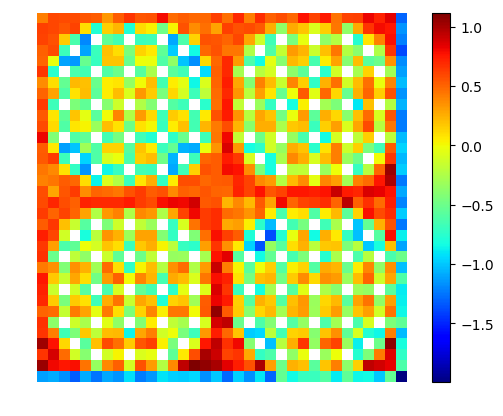
\includegraphics[width=\linewidth]{figures/reflector/capt-null-errors}
  \caption{}
  \label{fig:reflector-capt-null-error}
\end{subfigure}%
\begin{subfigure}{0.45\textwidth}
  \centering
  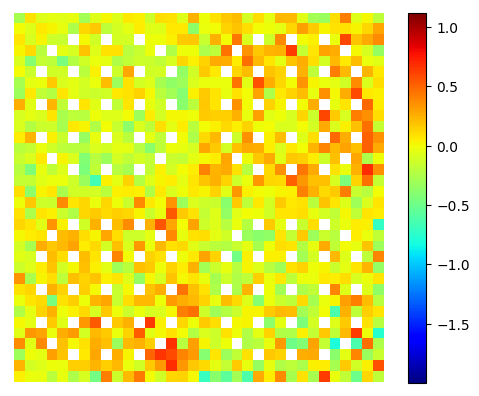
\includegraphics[width=\linewidth]{figures/reflector/capt-degenerate-errors}
  \caption{}
  \label{fig:reflector-capt-degen-error}
\end{subfigure}
\caption{OpenMOC U-238 capture rate percent relative errors for the assembly (a) and colorset (b) benchmarks.}
\label{fig:capt-errors}
\end{figure*}
